\chapter{数学知识总结}

\section{各类矩阵定义}

%%%%%%%%%%%%%%%%%%转置矩阵%%%%%%%%%%%%%%%%%%
\begin{definition}{\hypertarget{transpose}{转置矩阵}}{int}
\label{def:transpose}
把矩阵$A$的行换乘同序数的列得到一个新矩阵,就叫做$A$的转置矩阵,记作$A^{T}$。例如矩阵
\begin{align}
A = 
\begin{bmatrix}
1 & 2 & 0 \\
3 & -1 & 1
\end{bmatrix}
\end{align}
的转置矩阵为
\begin{align}
A^{T} = 
\begin{bmatrix}
1 & 3 \\
2 & -1 \\
0 & 1
\end{bmatrix}
\end{align}
\end{definition}

%%%%%%%%%%%%%%%%%%对称矩阵%%%%%%%%%%%%%%%%%%
\begin{definition}{\hypertarget{symmetric}{对称矩阵}}{int}
\label{def:symmetric}

设$A$为$n$阶方阵,如果满足$A^T=A$,即:
\begin{align}
a_{ij} = a_{ji}  (i,j=1, 2, ..., n)
\end{align}
那么$A$称为对称矩阵,简称为对称阵。对称阵的特点是:它的元素以对角线为对称轴对应相等。
\end{definition}

%%%%%%%%%%%%%%%%%%复共轭矩阵%%%%%%%%%%%%%%%%%%
\begin{definition}{\hypertarget{ctranspose}{复共轭矩阵}}{int}
\label{def:ctranspose}
设$A\in{C^{m\times{n}}}$,用$\bar{A}$表示以$A$的元素的共轭复数为元素组成的矩阵,命:
\begin{align}
A^{H} = (\bar{A})^{T}
\end{align}
则称$A^{H}$为$A$的复共轭转置矩阵。
\end{definition}



%%%%%%%%%%%%%%%%%%Hermitian矩阵%%%%%%%%%%%%%%%%%%
\begin{definition}{\hypertarget{hermitian}{Hermitian矩阵}}{int}
\label{def:hermitian}
设$A\in{R^{n\times{n}}}$,若$A^{H}=A$,则称$A$为Hermitian矩阵。若$A^{H}=-A$,则称$A$为反Hermitian矩阵。
\end{definition}

%%%%%%%%%%%%%%%%%%正交矩阵%%%%%%%%%%%%%%%%%%
\begin{definition}{\hypertarget{orthogonal}{正交矩阵}}{int}
\label{def:orthogonal}
如果$n$阶矩阵$A$满足
\begin{align}
A^{T}A=E
\end{align}
即:
\begin{align}
A^{T}=A^{-1}
\end{align}
则称$A$为正交矩阵,简称正交阵。
\end{definition}

%%%%%%%%%%%%%%%%%%酉矩阵%%%%%%%%%%%%%%%%%%
\begin{definition}{\hypertarget{unitary}{酉矩阵}}{int}
\label{def:unitary}
如果$n$阶复矩阵$A$满足
\begin{align}
A^{H}A=AA^{H}=E
\end{align}
则称$A$为酉矩阵,记作$A\in{U^{n\times{n}}}$。
\end{definition}

%%%%%%%%%%%%%%%%%%奇异矩阵%%%%%%%%%%%%%%%%%%
\begin{definition}{\hypertarget{singular}{奇异矩阵}}{int}
\label{def:singular}
当$|A|=0$时,$A$称为奇异矩阵,否则称为非奇异矩阵。$A$是可逆矩阵的充分必要条件是$|A|\neq{0}$,即可逆矩阵就是非奇异矩阵。
\end{definition}

%%%%%%%%%%%%%%%%%%正规矩阵%%%%%%%%%%%%%%%%%%
\begin{definition}{\hypertarget{formal}{正规矩阵}}{int}
\label{def:formal}
设$A\in{C^{n\times{n}}}$,若:
\begin{align}
A^{H}A=AA^{H}
\end{align}
则称$A$为正规矩阵,$A\in{R^{n\times{n}}}$,显然有$A^{H}=A^{T}$,上式就变成了:
\begin{align}
A^{T}A=AA^{T}
\end{align}
则称$A$为实正规矩阵。
\end{definition}

%%%%%%%%%%%%%%%%%%幂等矩阵%%%%%%%%%%%%%%%%%%
\begin{definition}{\hypertarget{power}{幂等矩阵}}{int}
\label{def:power}
设$A\in{C^{n\times{n}}}$,若:
\begin{align}
A^{2}=A
\end{align}
则称$A$是幂等矩阵。
\end{definition}

%%%%%%%%%%%%%%%%%%正定矩阵%%%%%%%%%%%%%%%%%%
\begin{definition}{\hypertarget{positive}{正定矩阵}}{int}
\label{def:positive}
设$A\in{C^{n\times{n}}}$,若A的所有特征值均为正数,则称$A$为正定矩阵;若$A$的特征值均为非负数,则称$A$为版正定矩阵。

判断一个矩阵为正定矩阵的充要条件有:
\begin{enumerate}
\item $A$的所有特征值$\lambda_{i}$均为正数;
\item $x^{T}Ax \ge 0$对所有非零向量$x$都成立;
\item 存在秩满矩阵$R$,使得$A=R^{T}R$。
\end{enumerate}
\end{definition}

\section{瑞利商}
\label{sec:rayleigh-quotient}
对于一个\hyperlink{hermitian}{Hermitian矩阵}$M$及非零向量$x$,\href{https://en.wikipedia.org/wiki/Rayleigh_quotient}{瑞利商}(Rayleigh quotient)的定义如公式\ref{eqn:ray1},其中$x^{H}$为$x$的共轭转置向量。
\begin{align}
\label{eqn:ray1}
R(M,x)=\frac{x^{H}Mx}{x^{H}x}
\end{align}

若$M$和$x$中元素均为实数,瑞利商可以写成公式\ref{eqn:ray2}。
\begin{align}
\label{eqn:ray2}
R(M,x)=\frac{x^{T}Mx}{x^{T}x}
\end{align}

设M的特征值与特征向量分别为$\lambda_1, ..., \lambda_n$和$v_1, .., v_n$,且满足 $\lambda_{\min}=\lambda_1\leq{\lambda_2}\leq{...}\leq{\lambda_n}=\lambda_{\max}$,那么在M已知的情况下有:
\begin{align}
\label{eqn:conc-ray}
\begin{split}
\mathop{\max}_{x}R(M,x) &= \lambda_{n} \\
\mathop{\min}_{x}R(M,x) &= \lambda_{1}
\end{split}
\end{align}

以下为证明公式\ref{eqn:conc-ray}的过程:

由于$M$是Hermitian矩阵,存在一个酉矩阵$U$,满足公式\ref{eqn:unity-matrix}。
\begin{align}
\label{eqn:unity-matrix}
M=UAU^{T}
\end{align}
其中$A=diag\{\lambda_1, ..., \lambda_n\}$。

因此公式\ref{eqn:ray2}可以转换如下:
\begin{align}
\begin{split}
R(M,x) &= \frac{x^{T}UAU^{T}x}{x^{T}x} \\
       &= \frac{(U^{T}x)^{T}A(U^{T}x)}{x^{T}x}  
\end{split}
\end{align}

设$P=U^{T}x$,则:
\begin{align}
\label{eqn:trans1}
\begin{split}
R(M,x) &= \frac{P^{T}AP}{x^{T}x} \\
       &= \frac{\sum_{i=1}^{n}\lambda_{i}|P_i|^{2}}{\sum_{i=1}^{n}|x_i|^{2}}
\end{split}
\end{align}

根据特征值的大小关系,我们可以得到不等式\ref{eqn:feature-unequal}。
\begin{align}
\label{eqn:feature-unequal}
\lambda_{1}\sum_{i=1}^{n}|P_i|^{2} \leq \sum_{i=1}^{n}\lambda_{i}|P_i|^{2} \leq \lambda_{n}\sum_{i=1}^{n}|P_i|^{2}
\end{align}

所以公式\ref{eqn:trans1}的范围如下:
\begin{align}
\label{eqn:trans0}
\lambda_{1}\frac{\sum_{i=1}^{n}|P_i|^{2}}{\sum_{i=1}^{n}|x_i|^{2}} \leq R(M,x) \leq \lambda_{n}\frac{\sum_{i=1}^{n}|P_i|^{2}}{\sum_{i=1}^{n}|x_i|^{2}} 
\end{align}

设$U$第$i$行第$j$列的元素为$u_{ij}$,则$U^{T}$第$i$行第$j$列的元素为$u_{ji}$,由$P=U^{T}x$和$P^{T}=x^{T}U$可得:
\begin{align}
\begin{split}
p_i &= \sum_{i=1}^{n} u_{ji}x_j \\
p_{i}^{T} &= \sum_{j=1}^{n} x_{i}u_{ij}
\end{split}
\end{align}

则:

\begin{align}
|p_i|^{2} = p_{i}^{T}p_i = \sum_{j=1}^{n} \sum_{k=1}^{n} x_j u_{ij} u_{ki} x_k
\end{align}

于是:
\begin{align}
\label{eqn:trans2}
\begin{split}
\sum_{i=1}^{n}|p_i|^{2} &= \sum_{i=1}^{n} p_{i}^{T}p_i \\
                        &= \sum_{i=1}^{n} \sum_{j=1}^{n} \sum_{k=1}^{n} x_j u_{ij} u_{ki} x_k \\
                        &= \sum_{j=1}^{n} \sum_{k=1}^{n} (\sum_{i=1}^{n} u_{ki} u_{ij}) x_j x_k 
\end{split}
\end{align}

因为$U$是酉矩阵,满足$U^{T}U=I$,所以:
\begin{align}
I_{jk} = \sum_{i=1}^{n} u_{ji} u_{ik}
\end{align}

其满足如下等式:
\begin{equation}
\label{eqn:trans3}
I_{jk}=\left\{
\begin{array}{rcl}
1 & & j = k\\
0 & & j \neq k
\end{array} \right
\end{equation}

结合\ref{eqn:trans2}和\ref{eqn:trans3}可得如下等式:
\begin{align}
\sum_{i=1}^{n}|p_i|^{2} = \sum_{i=1}^{n} |x_i|^2
\end{align}

代入公式\ref{eqn:trans0}可得:
\begin{align}
\label{eqn:trans4}
\lambda_{1} \leq R(M,x) \leq \lambda_{n} 
\end{align}
且:
\begin{equation}
\label{eqn:trans5}
R(M,x)=\left\{
\begin{array}{rcl}
\lambda_{1} & & x = v_1\\
\lambda_{n} & & x = v_n
\end{array} \right
\end{equation}

如果用$x^{'}=cx$代入公式\ref{eqn:ray2}有:
\begin{align}
\begin{split}
R(M,x^{'})  &=\frac{x^{'}^{T}Mx^{'}}{x^{'}^{T}x^{'}}  \\
            &=\frac{c^{2}x^{T}Mx}{c^{2}x^{T}x}  \\
            &=\frac{x^{T}Mx}{x^{T}x} 
\end{split}
\end{align}

由此可以看出来对$x$进行缩放不影响瑞利商的值,即:
\begin{align}
R(M,cx) = R(M,x) 
\end{align}

因此我们可以限定$x^Tx=1$,那么公式\ref{eqn:ray2}可以简化为:
\begin{align}
R(M,x) = x^{T}Mx
\end{align}

那么$R(M,x)$的极值就可以转换成约束条件下的拉格朗日乘法,如公式\ref{eqn:lage}。
\begin{align}
\label{eqn:lage}
L(x, \lambda) = x^{T}Mx - \lambda(x^{T}x-1)
\end{align}

对$x$求导并置为0可得:
\begin{align}
\nabla{L(x, \lambda)} = Mx - \lambda{x} = 0
\end{align}
即$M$的特征值能使得瑞利商取极值,且有:
\begin{align}
R(M,x) = \lambda
\end{align}

瑞利商可以推广至广义瑞利商(Generalized Rayleigh Quotient),其形式如公式\ref{eqn:GRQ}。
\begin{align}
\label{eqn:GRQ}
R(A,B,x) = \frac{x^{H}Ax}{x^{H}Bx}
\end{align}
其中$A$, $B$均为$n\times{n}$的Hermitian矩阵,且$B$为正定矩阵。

令$x=B^{-\frac{1}{2}}x^{'}$,广义瑞利商可以改写成:
\begin{align}
\label{eqn:GRQ}
\begin{split}
R(A,B,x) &= \frac{(B^{-\frac{1}{2}}x^{'})^{H}A(B^{-\frac{1}{2}}x^{'}))}{(B^{-\frac{1}{2}}x^{'})^{H}B(B^{-\frac{1}{2}}x^{'})} \\
         &= \frac{x^{'}^{H}(B^{-\frac{1}{2}})^{H}AB^{-\frac{1}{2}}x^{'}}{x^{'}^{H}(B^{-\frac{1}{2}})^{H}BB^{-\frac{1}{2}}x^{'}}  \\
         &= \frac{x^{'}^{H}(B^{-\frac{1}{2}})^{H}AB^{-\frac{1}{2}}x^{'}}{x^{'}^{H}x^{'}}
\end{split}
\end{align}

此时$R(A,B,x)$的最大特征值和最小特征值即为$(B^{-\frac{1}{2}})^{H}AB^{-\frac{1}{2}}$的最大和最小特征值。其实等价于当$M=(B^{-\frac{1}{2}})^{H}AB^{-\frac{1}{2}}$时的$R(M,x^{'})$,$x^{'}=B^{\frac{1}{2}}x$。

为简单起见,我们可以令$P=B^{-\frac{1}{2}}$,公式\ref{eqn:GRQ}可以写作:
\begin{align}
\label{eqn:GRQ1}
\begin{split}
R(A,B,x) &= \frac{x^{'}^{H}(B^{-\frac{1}{2}})^{H}AB^{-\frac{1}{2}}x^{'}}{x^{'}^{H}x^{'}} \\
         &= \frac{x^{'}^{H}P^{H}APx^{'}}{x^{'}^{H}x^{'}}  \\
         &= \frac{(Px^{'})^{H}APx^{'}}{x^{'}^{H}x^{'}}
\end{split}
\end{align}

类比上面提到的拉格朗日乘法,我们可以得到如下等式:
\begin{align}
\nabla{L(x, \lambda)} = P^{H}APx^{'} - \lambda{x^{'}} = 0
\end{align}

代入$x^{'}=P^{-1}x$有:
\begin{align}
\nabla{L(x, \lambda)} = P^{H}APP^{-1}x - \lambda{P^{-1}x} 
\end{align}

解得:
\begin{align}
PP^{H}Ax=\lambda{x} 
\end{align}

又因为$B^{-1}=PP^{H}$,所以最终求解特征值和特征向量可以依据:
\begin{align}
B^{-1}Ax=\lambda{x}
\end{align}

\section{混合高斯分布}

%%%%%%%%%%%%%%%%%%方差%%%%%%%%%%%%%%%%%%
\begin{definition}{方差}{int}
方差用于描述数据的离散或波动程度。假定变量为$X$,均值为$\bar{X}$,$N$为总体样本数,方差计算公式如下:
\begin{align}
var(X) = \frac{\sum_{i=1}^{N}(X_i-\bar{X})^{2}}{N-1}
\end{align}
\end{definition}

%%%%%%%%%%%%%%%%%%协方差%%%%%%%%%%%%%%%%%%
\begin{definition}{协方差}{int}
协方差表示了变量线性相关的方向,取值范围是$[-\infty, \infty]$,一般来说协方差为正值,说明一个变量变大另一个变量也变大;取负值说明一个变量变大另一个变量变小,取0说明两个变量没有相关关系.
\begin{align}
cov(X) = \frac{\sum_{i=1}^{N}(X_i-\bar{X})^{2}(Y_i-\bar{Y})^{2}}{N-1}
\end{align}
\end{definition}

%%%%%%%%%%%%%%%%%%相关系数%%%%%%%%%%%%%%%%%%
\begin{definition}{相关系数}{int}
协方差可反映两个变量之间的相互关系及相关方向,但无法表达其相关的程度,皮尔逊相关系数不仅表示线性相关的方向,还表示线性相关的程度,取值$[-1,1]$,也就是说,相关系数为正值,说明一个变量变大另一个变量也变大;取负值说明一个变量变大另一个变量变小,取0说明两个变量没有相关关系,同时,相关系数的绝对值越接近1,线性关系越显著。
\begin{align}
\rho_{XY} = \frac{cov(X, Y)}{\sqrt{DX}\sqrt{DY}}
\end{align}
\end{definition}

%%%%%%%%%%%%%%%%%%协方差矩阵%%%%%%%%%%%%%%%%%%
\begin{definition}{协方差矩阵}{int}
 当$X\in{R^{n}$为高维数据时,协方差矩阵可以很好的反映数据的性质,在协方差矩阵中,对角线元素反映了数据在各个维度上的离散程度,协方差矩阵为对角阵,非对角线元素反映了数据各个维度的相关性,其形式如下:
\begin{align}
\Sigma = 
\begin{bmatrix}
cov(x_1, x_1) & cov(x_1, x_2) & \cdots & cov(x_1, x_n) \\
cov(x_2, x_1) & cov(x_2, x_2) & \cdots & cov(x_2, x_n) \\
\vdots        & \vdots        & \ddots    & \vdots \\
cov(x_n, x_1) & cov(x_n, x_2) & \cdots & cov(x_n, x_n) 
\end{bmatrix}
\end{align}
\end{definition}

单变量高斯分布公式如\ref{eqn:gaussian},其中$\mu$和$\sigma^{2}$分别为均值和方差。
\begin{align}
\label{eqn:gaussian}
\mathcal{N}(x; \mu, \sigma) = \frac{1}{\sqrt{2\pi}\sigma}\exp{\{-\frac{(x-\mu)^{2}}{2\sigma^{2}}\}}
\end{align}

多变量高斯分布公式如\ref{eqn:mgaussian},其中$\mu$和$\Sigma$分别为均值和协方差矩阵。
\begin{align}
\label{eqn:mgaussian}
\mathcal{N}(x; \mu, \Sigma) = \frac{1}{(2\pi)^{-\frac{n}{2}}|\Sigma|^{\frac{1}{2}}}\exp{\{-\frac{1}{2}(x-\mu)^{T}\Sigma^{-1}(x-\mu)\}}
\end{align}

混合高斯模型(Gaussian Mixture Model)表示的是多个高斯分布叠加在一起的分布,其公式如\ref{eqn:GMM},其中$K$为高斯分量的个数,$\pi_{k}$为各个分量的权重,其满足$0 \leq \pi_{k} \leq 1$,且$\sum_{k=1}^{K}\pi_{k}=1$。$p(x)$表示的是多个高斯分量加权后的分布。
\begin{align}
\label{eqn:GMM}
p(x) = \sum_{k=1}^{K}\pi_{k}\mathcal{N}(x; \mu_{k}, \Sigma_{k})
\end{align}

\section{线性判别分析}
线性判别分析(Linear Discriminative Analysis, LDA)是一种有监督的降维学习方法,其不仅仅可以达到降维的目的,还可以对原始数据进行聚类,使得类间距变大,类内距变小。有监督意味着LDA中所有的数据都是有标签的,这也是和PCA的一个重要区别,PCA无需样本类别,是一种无监督的降维方法。

LDA概况起来就是“投影后类内方差最小,类间方差最大。”LDA是对数据进行投影,将其投影到低维空间,投影后相同类别的样本距离更近,不同类别的类别中心更远。本节首先对二类LDA进行分析,再推广至多类LDA。

二类LDA的形象表述如图\ref{fig:lda-bi}右。左边的图不同类之间有交叉,决策边界有重合,而右图既使得相同类更集中,也使得不同类的分类边界更清晰,这就是LDA达到的效果。
\begin{figure}[htbp]
  \centering
  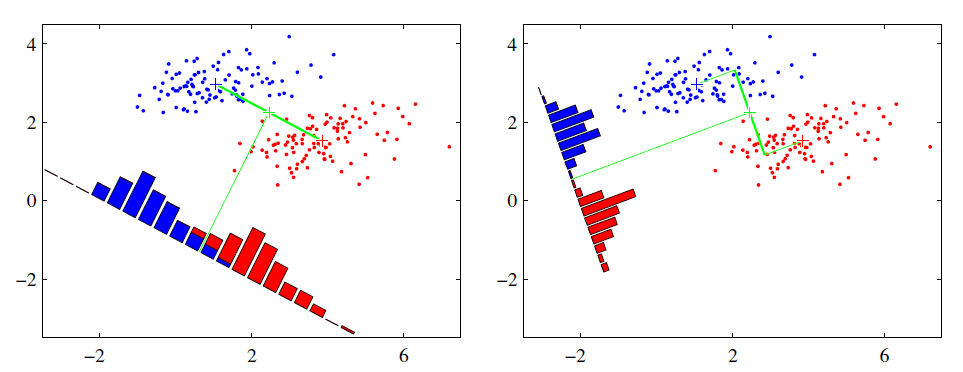
\includegraphics[width=0.55\textwidth]{lda-bi}
  \caption{二类LDA转换效果图 \label{fig:lda-bi}}
\end{figure}

假定数据集$D=\{(x_1, y_1), (x_2, y_2), ..., (x_m, y_m)\}$,其中$x_i \in R^{n}$,$y_i \in \{0, 1\}$。我们定义$N_j (j=0,1)$为第$j$类样本的个数,$X_j (j=0,1)$为第$j$类样本的合集,$\mu_j (i=0,1)$为第$j$类样本的均值向量,$\Sigma_j (j=0,1)$为第$j$类样本缺少分母部分的协方差矩阵。那么$\mu_j$和$\Sigma_j$的表达式分别如公式\ref{eqn:lda-mean}和公式\ref{eqn:lda-var}所示。
\begin{align}
\mu_j &= \frac{1}{N_j} \sum_{x\in{j}} x  \label{eqn:lda-mean}\\
\Sigma_j &= \sum_{x\in{j}} (x-\mu_{j})(x-\mu_{j})^{T} \label{eqn:lda-var}
\end{align}

由于只有两类数据,所以只需要将这些数据投影到一条直线上就可以,假设投影向量为$w$,则对任意一个样本,其在直线上的投影为$w^{T}x$,类别中心的投影分别为$w^{T}\mu_{0}$和$w^{T}\mu_{1}$,LDA要求不同类别之间的类别中心尽可能的远,所以需要最大化$\parallel w^{T}\mu_{0} - w^{T}\mu_{1} \parallel_{2}^{2}$,同时我们还希望同一类别尽可能接近,也就是样本投影之后的协方差尽可能的小,投影后的协方差如公式\ref{eqn:shadow-var}。
\begin{align}
\label{eqn:shadow-var}
\begin{split}
\Sigma_{j}^{'} &= \sum_{x\in{j}} (w^{T}x-w^{T}\mu_{j})(w^{T}x-w^{T}\mu_{j})^{T} \\
               &= \sum_{x\in{j}} w^{T}(x-\mu_{j})(x-\mu_{j})^{T}w \\
               &= w^{T}\Sigma_{j} w
\end{split}
\end{align}
所以我们希望最小化 $w^{T}\Sigma_{0} w + w^{T}\Sigma_{1} w$,由此我们可以得到需要优化的目标函数,如公式\ref{eqn:lda-obj-bi}。
\begin{align}
\label{eqn:lda-obj-bi}
\begin{split}
\arg\mathop{\max}_{w} J(w) &= \arg\mathop{\max}_{w}  \frac{\parallel w^{T}\mu_{0} - w^{T}\mu_{1} \parallel_{2}^{2}}{w^{T}\Sigma_{0} w + w^{T}\Sigma_{1} w} \\
                           &= \arg\mathop{\max}_{w}  \frac{w^{T} (\mu_{0} - \mu_{1}) (\mu_{0} - \mu_{1})^{T}w }{w^{T}(\Sigma_{0} + \Sigma_{1}) w} \
\end{split}
\end{align}

类内散度矩阵$S_w$和类间散度矩阵$S_b$分别定义为公式\ref{eqn:intra-matrix}和公式\ref{eqn:inter-matrix}。
\begin{align}
S_w &= \Sigma_{0} + \Sigma_{1} \label{eqn:intra-matrix}\\
S_b &= (\mu_{0} - \mu_{1}) (\mu_{0} - \mu_{1})^{T}  \label{eqn:inter-matrix}
\end{align}

所以目标函数就变成了:
\begin{align}
\label{eqn:lda-obj-bi-rui}
\arg\mathop{\max}_{w} J(w)  &= \arg\mathop{\max}_{w} \frac{w^{T}S_{b}w}{w^{T}S_{w}w} 
\end{align}

也就是求解出$w$使得$J(w)$最大。根据\ref{sec:rayleigh-quotient}中的介绍,我们可以通过计算矩阵$S_{w}^{-1}S_{b}$的特征值和特征向量得到对应的$w$,即求解公式\ref{eqn:lda-di-solve}。$J(w)$的最大值为$S_{w}^{-1}S_{b}$的最大特征值,最小值为$S_{w}^{-1}S_{b}$的最小特征值,而$S_w$和$S_b$均可由原始数据求解得出,因此很容易就可以求解出$J(w)$的最大值。
\begin{align}
\label{eqn:lda-di-solve}
S_{w}^{-1}S_{b}w = \lambda{w}
\end{align}

接下来我们分析下多类LDA的原理。

假定数据集$D=\{(x_1, y_1), (x_2, y_2), ..., (x_m, y_m)\}$,其中$x_i \in R^{n}$,$y_i \in \{C_1, C_2, ..., C_k\}$。我们定义$N_j (j=0,1,...,k)$为第$j$类样本的个数,$X_j (j=0,1,...,k)$为第$j$类样本的合集,$\mu_j (i=0,1,...,k)$为第$j$类样本的均值向量,$\Sigma_j (j=0,1,...,k)$为第$j$类样本缺少分母部分的协方差矩阵。此时是多类分类,因此投影后的空间不再是一条直线,而是一个超平面。假设投影后的低维空间维度为$d$,对应的基向量为$(w_1, w_2,..., w_d)$,基向量组成的矩阵为$W\in{R^{n*d}}$。

此时类内的散度矩阵$S_W$仍旧存在,如公式\ref{eqn:intra-multi}。
\begin{align}
\label{eqn:intra-multi}
S_W = \sum_{j=1}^{k} \Sigma_{j} 
\end{align}

但是类间的散度矩阵就有所不同了。此时用每个类别的均值到全局均值的距离来衡量类间距如图\ref{fig:lda-mul}。
\begin{figure}[htbp]
  \centering
  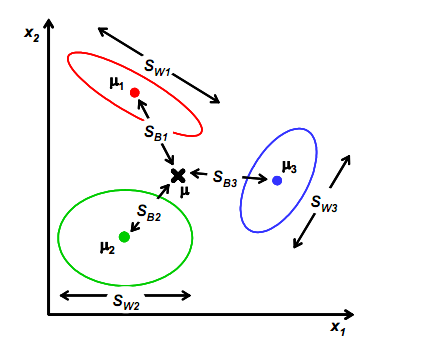
\includegraphics[width=0.55\textwidth]{lda-mul}
  \caption{多类LDA的类间散度矩阵示意图 \label{fig:lda-mul}}
\end{figure}

其定义为公式\ref{eqn:inter-multi}。
\begin{align}
\label{eqn:inter-multi}
S_B = \sum_{j=1}^{k} N_j (\mu_{j} - \mu)(\mu_{j} -\mu)^{T}
\end{align}
其中:
\begin{align}
\mu     &= \frac{1}{m}\sum_{i=1}^{m} x_{i} \\
\mu_{j} &= \frac{1}{N_{j}}\sum_{x_{j}\in{C_{j}}} x_{j}
\end{align}

同样此时的优化目标为公式\ref{eqn:lda-obj-multi}。
\begin{align}
\label{eqn:lda-obj-multi}
\arg\mathop{\max}_{W} J(W)  &= \arg\mathop{\max}_{W} \frac{W^{T}S_{B}W}{W^{T}S_{W}W} 
\end{align}

此时目标函数求解转换成了公式\ref{eqn:lda-mul-solve}:
\begin{align}
\label{eqn:lda-mul-solve}
S_{W}^{-1}S_{B}W = \lambda{W}
\end{align}

以上,可以总结出多类LDA的求解步骤:
\begin{enumerate}
  \item 计算每个类别的均值向量和方差,以及全局均值向量;
  \item 根据均值向量和方差,计算$S_w$和$S_B$;
  \item 对$S_{W}^{-1}S_{B}W = \lambda{W}$进行求解,求出$S_{W}^{-1}S_{B}$的特征值和特征向量;
  \item 对特征向量进行排序,设定低维空间的维度$d$,选取前$d$个特征值和特征向量,特征向量组合成投影矩阵$W$;
  \item 通过投影矩阵计算出投影后的输入数据$x_{i}^{'}=W^{T}x_{i}$;
  \item 得到输出的新数据集:$\{(x_{1}^{'}, y_1), (x_{2}^{'}, y_2), ..., (x_{m}^{'}, y_m)\}$。
\end{enumerate}

\section{EM算法}
\label{sec:em}
本节来自于Andrew Ng的课堂讲义\upcite{em-alg}以及李航老师的《统计学习方法》\upcite{stat-lihang}。

\subsection{Jensen's Inequality}
首先介绍一下\href{https://en.wikipedia.org/wiki/Jensen\%27s_inequality}{Jensen不等式}。



一般地,用$Y$表示观测随机变量的数据,$Z$表示隐随机变量的数据,$Y$和$Z$连在一起称为完全数据。观测数据$Y$又称为不完全数据。假设给定观测数据$Y$,其概率分布是$P(Y|\theta)$,其中$\theta$是需要估计的参数,那么不完全数据$Y$的似然函数是$P(Y|\theta)$,对数似然函数是$L(\theta)=\log P(Y|\theta)$;假设$Y$和$Z$的联合概率分布是$P(Y,Z|\theta)$,那么完全数据的对数似然函数是$L(\theta)=\log P(Y,Z|\theta)$。

EM算法通过迭代求$L(\theta)=\log P(Y|\theta)$的极大似然估计,每次迭代分为两步:E步,求期望;M步,求极大化。

输入:观测变量数据$Y$,隐变量数据$Z$,联合分布$P(Y,Z|\theta)$,条件分布$P(Z|Y,\theta)$

\section{最大似然线性变换}
最大似然线性变换(Maximum Likelihood Linear Transform)

在HMM系统中,协方差矩阵的选择可以是对角阵,分块对角阵或者全矩阵。相对于对角阵来说,全矩阵的优势在于对特征向量元素之间关系的建模,劣势在于参数量巨大。

\section{Beta分布}
  

\section{MLE和MAP}

\href{https://wiseodd.github.io/techblog/2017/01/01/mle-vs-map/}{MLE vs MAP}

